%\documentstyle[epsf,twocolumn]{jarticle}       %LaTeX2e仕様
\documentclass[twocolumn]{jarticle}     %pLaTeX2e仕様(platex.exeの場合)
%\documentclass[twocolumn]{ujarticle}     %pLaTeX2e仕様(uplatex.exeの場合)
%%%%%%%%%%%%%%%%%%%%%%%%%%%%%%%%%%%%%%%%%%%%%%%%%%%%%%%%%%%%%%
%%
%%  基本バージョン
%%
%%%%%%%%%%%%%%%%%%%%%%%%%%%%%%%%%%%%%%%%%%%%%%%%%%%%%%%%%%%%%%%%
\setlength{\topmargin}{-45pt}
%\setlength{\oddsidemargin}{0cm} 
\setlength{\oddsidemargin}{-7.5mm}
%\setlength{\evensidemargin}{0cm} 
\setlength{\textheight}{24.1cm}
%setlength{\textheight}{25cm} 
\setlength{\textwidth}{17.4cm}
%\setlength{\textwidth}{172mm} 
\setlength{\columnsep}{11mm}

\kanjiskip=.07zw plus.5pt minus.5pt


% 【節が変わるごとに (1.1)(1.2) … (2.1)(2.2) と数式番号をつけるとき】
%\makeatletter
%\renewcommand{\theequation}{%
%\thesection.\arabic{equation}} %\@addtoreset{equation}{section}
%\makeatother

%\renewcommand{\arraystretch}{0.95} 行間の設定

%%%%%%%%%%%%%%%%%%%%%%%%%%%%%%%%%%%%%%%%%%%%%%%%%%%%%%%%
\usepackage[dvipdfmx]{graphicx}   %pLaTeX2e仕様(\documentstyle ->\documentclass)\documentclass[dvipdfmx]{graphicx}
\usepackage[dvipdfmx]{color}
\usepackage[subrefformat=parens]{subcaption}
\usepackage{colortbl}
\usepackage{multicol}
%%%%%%%%%%%%%%%%%%%%%%%%%%%%%%%%%%%%%%%%%%%%%%%%%%%%%%%%

\begin{document}

\twocolumn[
\noindent

\hspace{1em}
\today
\hfill
\ \ 細川 岳大

\vspace{2mm}

\hrule

\begin{center}
{\Large \bf 進捗報告}
\end{center}
\hrule
\vspace{3mm}
]

% ‚ここから 文章 Start!

\section{今週やったこと}
 GAを用いたDataAugmentaion

\section{実験}

\subsection{実験データ}
実験データはcifar10を用いて,
事前学習ではepoch数150,train\_dataを各ラベル4000枚の計40000枚使用し,GAで学習する際はepoch数30,train\_dataは各ラベル200枚のオリジナルとそれらすべてをDataAugmentaionしたものとを合わせ計4000枚とし,test\_data及びvalidation\_dataは共に10000枚とした.また事前学習でのaccuracyは0.8281である.
\subsection{分散遺伝的アルゴリズム}
多様性維持として分散遺伝的アルゴリズム(Distributed Genetic Algorithm:DGA)\cite{廣安知之2002実験計画法を用いた分散遺伝的アルゴリズムのパラメータ推定}を用いる.

\subsubsection{DGAの概要}
まず,GAの母集団を複数に分割をする.この分割されたものをサブ母集団といい,GAの遺伝子操作をサブ母集団ごとに施すことで,サブ母集団同士で多様性を維持することができる.\\
一方でサブ母集団は母集団よりも個体数が少なくなるため,初期収束が起こりやすくなる.
そこで探索情報を共有するために次項で説明する移住(Migration)という操作を用いる.


\subsubsection{移住}
移住はある一定の間隔でサブ母集団内の一部の個体を他のサブ母集団内の一部の個体と交換する操作である.
移住の間隔を移住間隔(Migration interval),交換する個体数の割合を移住率(Migration rate)という.
移住はGAの選択,交叉,突然変異という操作のうち,選択と交叉の間で行われるものとした.
また,今回移住先の制約として,移住元と移住先をすべてつなげた時にリング状のグラフになるようにした.また移住個体は
ランダムに選択するものとした.\\


\subsubsection{個体}
\ これまでと同様16の操作に対し強度,確率,順序をもった個体とする.

\subsubsection{選択}
\ 選択について,エリート選出によって最も適応度の高い2つの個体を選択する.なお,この二つは後述する交叉,突然変異は受けずに次の世代に追加する.
残りの選出にはトーナメント選出を用した.トーナメント選出は集団の中から任意の数(トーナメントサイズ)の個体のうち最も適応度の高い個体を選出し次の世代に追加する.今回トーナメントサイズは2とした.
 
\subsubsection{交叉}
\ 強度,確率を表す染色体については2点交叉,順序を表す染色体については部分写像交叉を用いた.2点交叉は一対の親染色体をそれぞれ同じ場所で三分割し中央の染色体を入れ替えて交叉を行う
 
\subsubsection{突然変異}
\ 強度,確率を表す染色体について,対象となる遺伝子の値を各50\%の確率に1増減させ,
 順序を表す染色体について,染色体の一部を逆順にする操作か,染色体を二つに分け前後を入れ替える操作のいずれかを行うものとした.
\subsection{適応度}
\ validation\_dataについてtargetとなる個体から得られた出力と,
その個体の属するサブ母集団以外の個体全ての出力で比較し,
targetで正答したものの中で,他の個体で誤答した問題数をカウントして適応度とした.

\subsection{アンサンブル学習}
\ 今回はサブ母集団ごとにもっとも適応度の高い個体を選び,それらをアンサンブルさせた.

\subsection{実験} 
\subsubsection{パラメータ}
表\ref{tb:param1}に学習パラメータを示す.
\begin{table}[h]
	\centering
	\caption{学習パラメータ\label{tb:param1}}
	\scalebox{1.0}{
		\begin{tabular}{|c||c|} \hline
			optimizer&Adam\\ \hline
			learning rate&0.001\\ \hline
			loss function&categorical\_crossentropy\\ \hline
			batch size&128\\ \hline
			epoch size&30\\ \hline
		\end{tabular}
	}
\end{table}
表\ref{tb:param_GA}にGAの設定を示す.
\begin{table}[h]
	\centering
	\caption{実験パラメータ\label{tb:param_GA}}
	\scalebox{1.0}{
		\begin{tabular}{|c|c|c|} \hline
			サブ母集団&個体数&10\\ \cline{2-3}
			&個数&10\\ \hline
			\multicolumn{2}{|c|}{総個体数}&100\\ \hline\hline
			\multicolumn{2}{|c|}{移住間隔}&3世代ごと\\ \hline
			\multicolumn{2}{|c|}{移住個体数}&3\\ \hline
			\multicolumn{2}{|c|}{世代数}&26\\ \hline
			\multicolumn{2}{|c|}{交叉率}&0.9\\ \hline\hline
			\multicolumn{3}{|c|}{突然変異率}\\ \hline
			\multicolumn{2}{|c|}{強度,確率(遺伝子ごと)}&0.06\\ \hline
			\multicolumn{2}{|c|}{順序(染色体ごと)}&0.1\\ \hline
		\end{tabular}
	}
\end{table}
\subsubsection{結果}
図\ref{fig:graph3},\ref{fig:graph3}に26世代目の遺伝子座をtSNEで次元圧縮したものを示す.
また,図\ref{fig:graph},\ref{fig:graph2},にvalとtestの推移を示す\\
また,train\_dataを全4000枚使用したものについてtestのaccuracyは1世代目が0.8901,26世代目が0.8947となった.

%\begin{figure}[h]
%	\centering
%	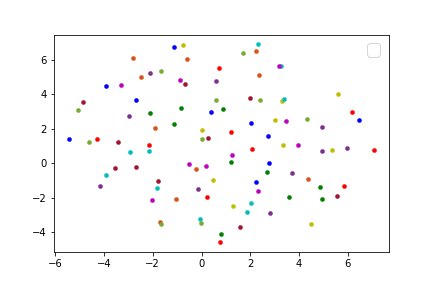
\includegraphics[scale=0.4]{graph0.png}
%	\caption{1世代目のtSNE図\label{fig:grap0}}
%\end{figure}

\begin{figure}[h]
	\centering
	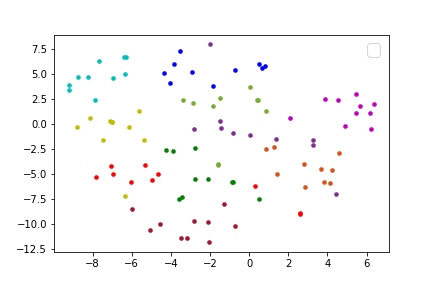
\includegraphics[scale=0.7]{graph3.png}
	\caption{26世代目の遺伝子座に対するtSNE図\label{fig:graph3}}
\end{figure}



\begin{figure}[hp]
	\centering
	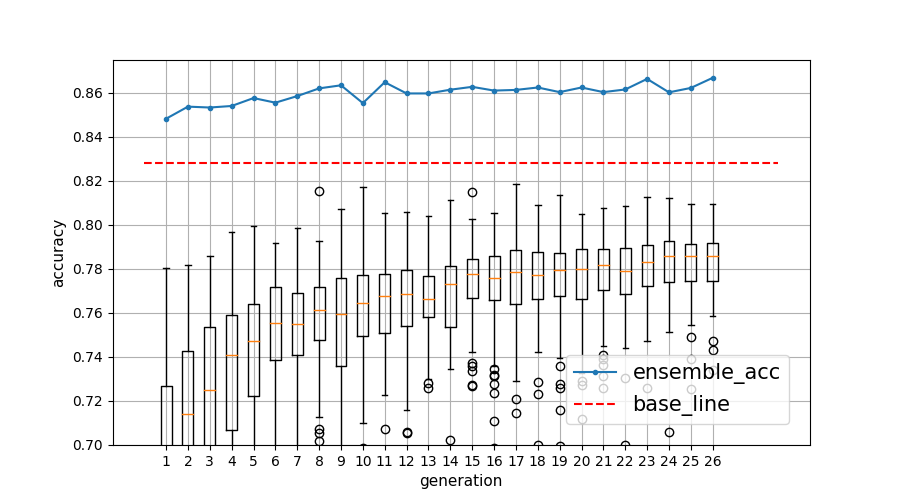
\includegraphics[scale=0.7]{graph1.png}
	\caption{valの推移\label{fig:graph}}
\end{figure}

\begin{figure}[hp]
	\centering
	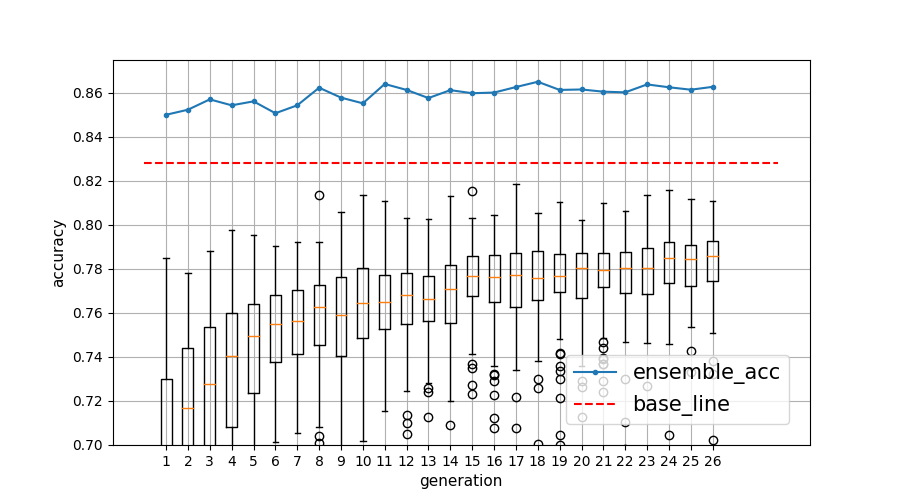
\includegraphics[scale=0.7]{graph2.png}
	\caption{testの推移\label{fig:graph2}}
\end{figure}


\subsection{まとめ}
\ アンサンブル学習自体はうまくいっている気もするが,初期世代と最終世代であまり大差がない.つまり,アンサンブルのなす多様性がDataAugmentationではなく学習時に絞ったデータの分配に起因していると考えらえる.DataAugmentationの違いでアンサンブルをすることの有用性を確認するためには学習のデータもすべて揃えなけばならないのではと思った.もしくは本当に現在の操作だけではアンサンブルに寄与するほどのことものではないかである.
\section{来週の課題}
\begin{itemize}
	\item 本当にDataAugmentationがアンサンブルに有効か確認する
	\item 絵本についてのリサーチを進める
\end{itemize}

\bibliography{sa}
\bibliographystyle{unsrt}

\end{document}


